% !TeX encoding = UTF-8
\chapter{Referencial teórico}
\label{cap:fund_teorico}

Este capítulo fundamenta os conceitos teóricos e técnicos necessários para a compreensão, execução e análise crítica da pesquisa proposta. A estrutura parte da apresentação das normas e dos mecanismos que regem a conectividade sem fio no padrão IEEE 802.11, com ênfase na camada de enlace e em seus mecanismos de acesso ao meio. Em seguida, analisa-se a arquitetura de ferramentas de \textit{hardware} ofensivo de baixo custo, em especial plataformas baseadas em microcontroladores. Por fim, discute-se o impacto técnico e sistêmico dessas vulnerabilidades no ecossistema da Internet das Coisas (IoT), com foco em ambientes residenciais. Todo o embasamento apresentado ancora-se no estado da arte da literatura acadêmica sobre segurança de redes, protocolos de comunicação e engenharia de microcontroladores \cite{KohliosHayajneh2018,Amoordon2022,Hiertz2010,Lima2025}.

\section{Segurança em redes sem fio e o protocolo IEEE 802.11}

\subsection{Evolução das normas e arquitetura da camada MAC}

O padrão IEEE 802.11, ratificado em 1997 pelo Instituto de Engenheiros Eletricistas e Eletrônicos (IEEE), estabeleceu as bases das redes locais sem fio (\textit{Wireless Local Area Networks} – WLAN) modernas. Sua evolução foi fortemente impulsionada pela necessidade de suportar volumes crescentes de tráfego de dados, mantendo a mobilidade dos nós e a flexibilidade de expansão das infraestruturas de telecomunicações \cite{Hiertz2010}. Nesse contexto, as primeiras emendas priorizaram o uso de faixas de radiofrequência não licenciadas, em especial as bandas ISM (\textit{Industrial, Scientific and Medical}) de 2{,}4~GHz e 5~GHz, e a melhoria progressiva da eficiência espectral e das taxas de transferência.

Do ponto de vista arquitetural, o IEEE 802.11 se apoia, principalmente, nas duas camadas inferiores do modelo de referência \textit{Open Systems Interconnection} (OSI): a camada física (PHY) e a camada de controle de acesso ao meio (MAC). Na camada física, \citeonline{Hiertz2010} descrevem a transição de esquemas de espectro espalhado relativamente simples e robustos a interferências, como o \textit{Direct Sequence Spread Spectrum} (DSSS) e o \textit{Frequency Hopping Spread Spectrum} (FHSS) do padrão original, de 1997, e o DSSS de alta taxa (HR/DSSS, \textit{High Rate DSSS}) da emenda 802.11b, para técnicas de modulação digital mais sofisticadas. O \textit{Orthogonal Frequency-Division Multiplexing} (OFDM), introduzido na emenda 802.11a, na faixa de 5~GHz, e levado aos 2,4~GHz pela emenda 802.11g, permitiu a divisão do sinal em múltiplas subportadoras ortogonais, aumentando significativamente a taxa efetiva de transmissão. Em seguida, a adoção de arranjos de múltiplas antenas (MIMO – \textit{Multiple-Input Multiple-Output}) a partir da emenda 802.11n viabilizou múltiplos fluxos espaciais em paralelo, elevando as taxas teóricas de aproximadamente 11~Mbit/s para patamares que podem ultrapassar a ordem de gigabits por segundo em versões mais recentes, como a 802.11ac \cite{Hiertz2010}.

Na camada MAC, por sua vez, a complexidade do protocolo reflete os desafios inerentes à transmissão pelo ar, um meio de difusão compartilhado, ruidoso e sujeito a colisões. Diferentemente das redes cabeadas baseadas em Ethernet (IEEE~802.3), que utilizam o mecanismo de detecção de colisões (CSMA/CD), o ambiente de radiofrequência impede que um nó perceba colisões de forma confiável enquanto transmite, devido à atenuação do sinal, ao efeito do nó oculto e ao fato de o transmissor mascarar sua própria recepção. Para contornar essa limitação, o IEEE 802.11 adota a \textit{Distributed Coordination Function} (DCF), responsável por implementar o mecanismo CSMA/CA (\textit{Carrier Sense Multiple Access with Collision Avoidance}) \cite{Hiertz2010}.

Nesse modelo, o dispositivo que deseja transmitir deve “escutar antes de falar” (\textit{listen-before-talk}), monitorando o meio antes de iniciar o envio de quadros. Se o canal permanecer livre por um intervalo denominado \textit{Distributed Interframe Space} (DIFS), a transmissão é iniciada; caso contrário, o dispositivo aguarda a liberação do meio e aplica um algoritmo de recuo exponencial (\textit{exponential backoff}) para reduzir a probabilidade de colisões subsequentes \cite{Hiertz2010}. Tal abordagem é fundamental para evitar a corrupção de quadros e garantir um nível mínimo de equidade no acesso ao meio. Entretanto, ela exige uma intensa troca de quadros de controle e de gestão para coordenar o acesso ao canal, de modo que a estabilidade da rede passa a depender diretamente da integridade e da autenticidade dessas mensagens de coordenação.

A Figura~\ref{fig:csma_ca} ilustra, de forma esquemática, o mecanismo CSMA/CA: a estação verifica o meio, aguarda o intervalo DIFS e, havendo disputa, aplica um recuo aleatório (\textit{backoff}) antes de transmitir o quadro, recebendo em seguida a confirmação (ACK) após um intervalo SIFS \cite{Hiertz2010}.

\begin{figure}[htb]
\centering
\caption{Mecanismo de acesso ao meio CSMA/CA com DIFS e \textit{backoff}}
\label{fig:csma_ca}
\resizebox{\textwidth}{!}{%
\begin{tikzpicture}[font=\small, seg/.style={draw, minimum height=10mm, align=center}]
\node[seg, fill=gray!20, minimum width=24mm] (busy) {Meio\\ocupado};
\node[seg, fill=blue!10, minimum width=16mm, right=0pt of busy] (difs) {DIFS};
\node[seg, fill=orange!18, minimum width=30mm, right=0pt of difs] (bo) {Janela de\\contenção\\(\textit{backoff})};
\node[seg, fill=green!15, minimum width=34mm, right=0pt of bo] (tx) {Transmissão\\do quadro};
\node[seg, fill=blue!10, minimum width=20mm, right=0pt of tx] (ack) {SIFS\\+ ACK};
\draw[-{Stealth}] ([yshift=-5mm]busy.south west) -- ([yshift=-5mm]ack.south east) node[below left]{tempo};
\end{tikzpicture}}
\legend{Fonte: elaborado pelo autor com base em Hiertz et al. (2010).}
\end{figure}

Ao longo das diversas emendas publicadas, a família 802.11 priorizou, de forma recorrente, ganhos de taxa de transmissão e de eficiência espectral em detrimento de uma preocupação inicial mais robusta com segurança. Emendas como 802.11b, 802.11g e 802.11n expandiram o uso de DSSS, OFDM e MIMO para atender à demanda crescente por aplicações multimídia, consolidando o Wi‑Fi como tecnologia predominante em ambientes residenciais e corporativos \cite{Hiertz2010}. Nesse processo, porém, a proteção das tramas de gerenciamento permaneceu limitada, o que resultou em uma base instalada de dispositivos com alta capacidade de transmissão, mas com superfícies de ataque relevantes ainda abertas na camada MAC, especialmente em relação à ausência de autenticação e integridade em quadros críticos de gestão \cite{KohliosHayajneh2018}.

A evolução temporal dos principais marcos da família IEEE~802.11 é sintetizada na Figura~\ref{fig:linha_tempo_80211}. A representação evidencia que o padrão foi ampliado para contemplar novas demandas de desempenho, interoperabilidade e segurança \cite{Hiertz2010}.

\begin{figure}[htb]
\centering
\caption{Principais marcos da evolução do padrão IEEE 802.11}
\label{fig:linha_tempo_80211}
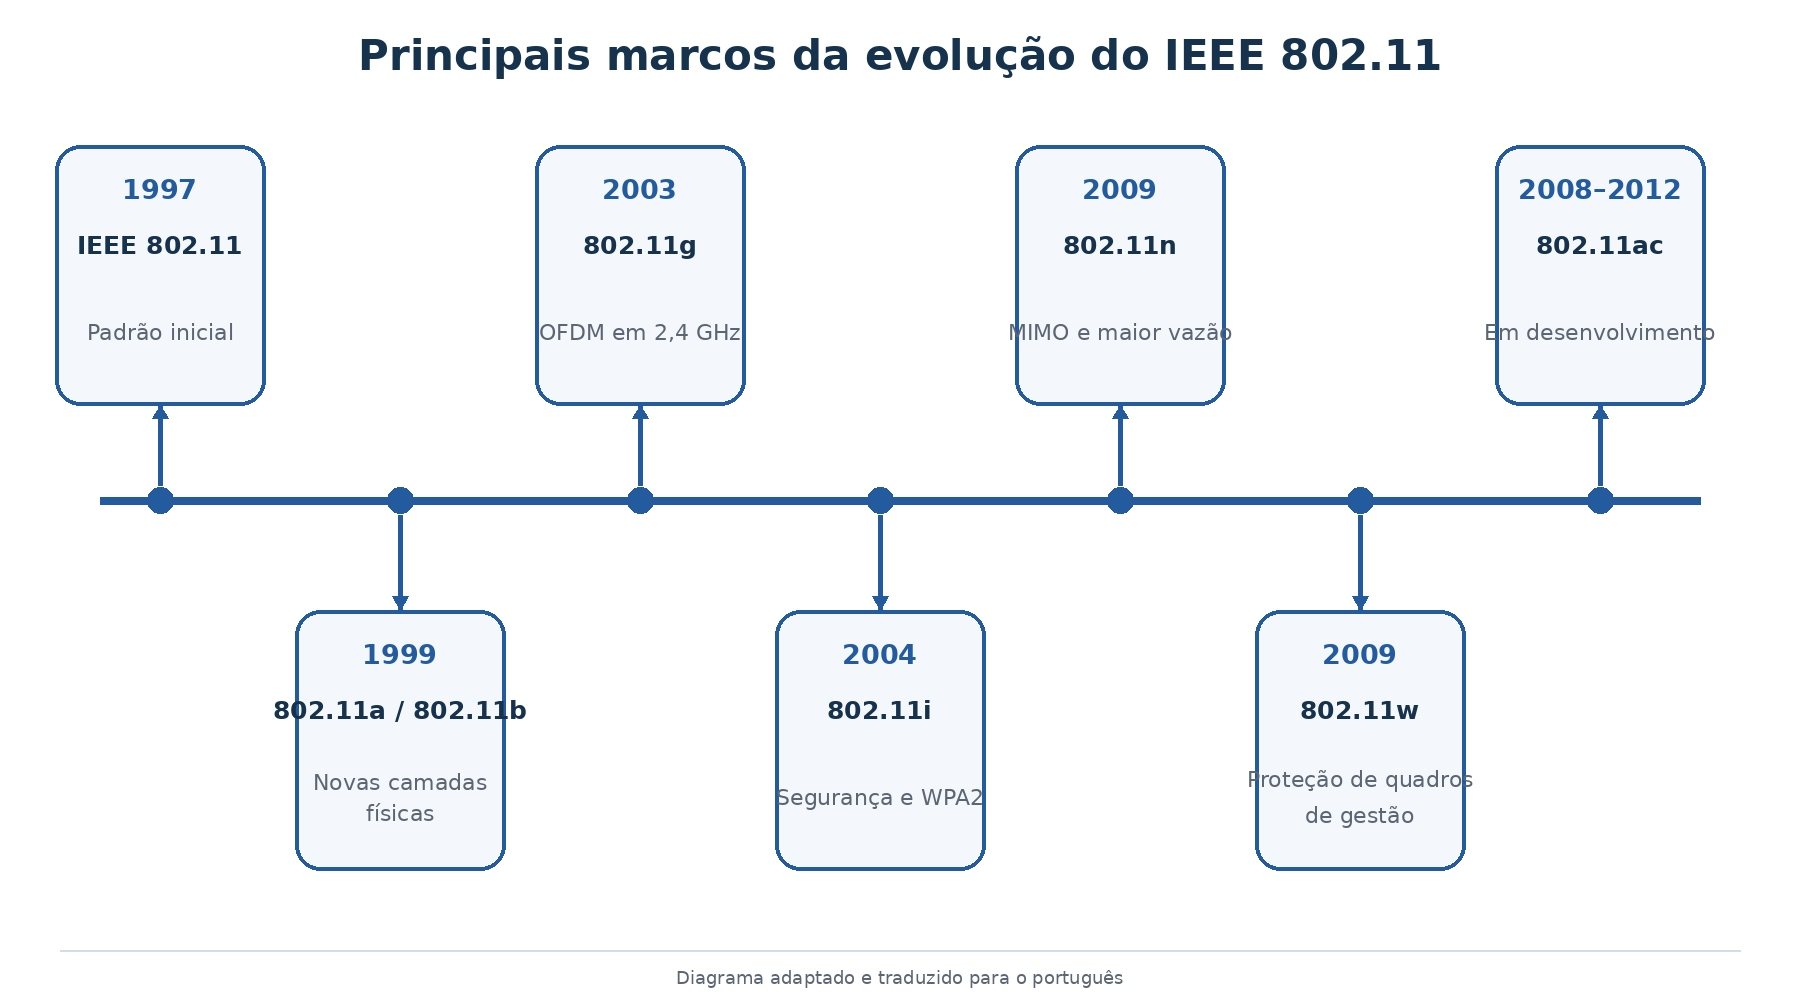
\includegraphics[width=0.96\textwidth]{linha_tempo_80211}
\legend{Fonte: adaptado de Hiertz et al. (2010).}
\end{figure}

Complementarmente à linha do tempo, a Figura~\ref{fig:emendas_mac_80211} organiza por área funcional as emendas do padrão, evidenciando os ramos de segurança (WEP, WPA, WPA2 e as emendas 802.11i e 802.11w), de qualidade de serviço (DCF; \textit{Point Coordination Function}, PCF; \textit{Hybrid Coordination Function}, HCF; e 802.11e) e de desempenho da camada física (802.11n, entre outras). Essa visão reforça que a proteção dos quadros de gerenciamento surge tardiamente na evolução do padrão, somente com a emenda 802.11w, o que é diretamente relevante para o objeto deste trabalho \cite{Hiertz2010,KohliosHayajneh2018}. Como \citeonline{Hiertz2010} é anterior ao WPA3, a inclusão desse ramo na figura apoia-se em \citeonline{KohliosHayajneh2018} e \citeonline{CiscoMFP2024}.

\begin{figure}[htb]
\centering
\caption{Emendas do padrão IEEE 802.11 organizadas por área funcional}
\label{fig:emendas_mac_80211}
\resizebox{\textwidth}{!}{%
\begin{tikzpicture}[font=\small, >=Stealth,
  n/.style={draw, rounded corners, minimum width=30mm, minimum height=8mm, align=center},
  hdr/.style={draw, rounded corners, minimum width=34mm, minimum height=9mm, align=center, font=\bfseries}]
\node[hdr, fill=blue!12] (root) at (0,2.2) {IEEE 802.11 (1997)};
\node[hdr, fill=orange!20] (seg) at (-5.6,0.6) {Segurança};
\node[hdr, fill=green!15] (qos) at (0,0.6) {QoS / Coordenação};
\node[hdr, fill=blue!10] (phy) at (5.6,0.6) {Desempenho (PHY)};
\draw[->] (root) -- (seg);
\draw[->] (root) -- (qos);
\draw[->] (root) -- (phy);
\node[n, fill=orange!8] (wep) at (-5.6,-0.6) {WEP};
\node[n, fill=orange!8] (wpa) at (-5.6,-1.7) {WPA (TKIP)};
\node[n, fill=orange!8] (wpa2) at (-5.6,-2.8) {WPA2 (802.11i)};
\node[n, fill=orange!8] (w11) at (-5.6,-3.9) {802.11w (PMF)};
\node[n, fill=orange!8] (wpa3) at (-5.6,-5.0) {WPA3 (SAE)};
\draw[->] (seg) -- (wep); \draw[->] (wep) -- (wpa); \draw[->] (wpa) -- (wpa2); \draw[->] (wpa2) -- (w11); \draw[->] (w11) -- (wpa3);
\node[n, fill=green!8] (dcf) at (0,-0.6) {DCF / PCF};
\node[n, fill=green!8] (hcf) at (0,-1.7) {HCF (HCCA/EDCA)};
\node[n, fill=green!8] (e11) at (0,-2.8) {802.11e};
\draw[->] (qos) -- (dcf); \draw[->] (dcf) -- (hcf); \draw[->] (hcf) -- (e11);
\node[n, fill=blue!6] (b11) at (5.6,-0.6) {802.11b (DSSS)};
\node[n, fill=blue!6] (g11) at (5.6,-1.7) {802.11g (OFDM)};
\node[n, fill=blue!6] (n11) at (5.6,-2.8) {802.11n (MIMO)};
\node[n, fill=blue!6] (ac11) at (5.6,-3.9) {802.11ac};
\draw[->] (phy) -- (b11); \draw[->] (b11) -- (g11); \draw[->] (g11) -- (n11); \draw[->] (n11) -- (ac11);
\end{tikzpicture}}
\legend{Fonte: elaborado pelo autor com base em Hiertz et al. (2010), para as emendas até 802.11ac, e em \citeonline{KohliosHayajneh2018} e \citeonline{CiscoMFP2024}, para 802.11w e WPA3.}
\end{figure}

\subsection{Tramas de gestão e a ausência de criptografia nativa}

A comunicação na camada MAC do protocolo IEEE 802.11 não se restringe ao transporte do tráfego gerado pelas aplicações dos usuários. O tráfego é organizado em três classes principais de quadros (\textit{frames}): quadros de dados, quadros de controle e quadros de gestão (\textit{management frames}). Os quadros de dados carregam a carga útil (\textit{payload}) proveniente das camadas superiores; os quadros de controle incluem, por exemplo, confirmações de recebimento (ACK) e sinais de coordenação de acesso ao meio, como \textit{Request to Send/Clear to Send} (RTS/CTS); por fim, os quadros de gestão são responsáveis por funções como descoberta de redes, sincronização e estabelecimento ou encerramento de associações \cite{Amoordon2022}.

A organização dos quadros nessas três classes é sintetizada na Figura~\ref{fig:classes_quadros}, na qual se destacam os quadros de gestão, foco deste trabalho por concentrarem as tramas de desautenticação e dissociação \cite{Amoordon2022,KohliosHayajneh2018}.

\begin{figure}[htb]
\centering
\caption{Classes de quadros da camada MAC do IEEE 802.11}
\label{fig:classes_quadros}
\begin{tikzpicture}[font=\small, every node/.style={align=center},
   box/.style={draw, rounded corners, minimum height=12mm, minimum width=32mm}]
\node[box, fill=gray!10] (root) at (0,0) {Quadros\\IEEE 802.11};
\node[box, fill=blue!8] (dados) at (-4.8,-2.4) {Dados\\(\textit{payload})};
\node[box, fill=blue!8] (ctrl) at (0,-2.4) {Controle\\(ACK, RTS/CTS)};
\node[box, fill=orange!20, minimum height=18mm] (gest) at (4.8,-2.4) {Gestão\\(\textit{beacon}, \textit{probe},\\autenticação, associação,\\\textbf{desautenticação}, dissociação)};
\draw[-{Stealth}] (root) -- (dados);
\draw[-{Stealth}] (root) -- (ctrl);
\draw[-{Stealth}] (root) -- (gest);
\end{tikzpicture}
\legend{Fonte: elaborado pelo autor com base em Amoordon et al. (2022) e Kohlios e Hayajneh (2018).}
\end{figure}

Segundo \citeonline{Amoordon2022}, os quadros de gestão constituem a espinha dorsal da conectividade sem fio, pois coordenam processos essenciais como autenticação e associação de estações (\textit{stations}, STA) a um ponto de acesso (AP – \textit{Access Point}). Entre os subtipos mais comuns, destacam‑se os \textit{beacons}, anúncios periódicos emitidos pelo AP que informam sua presença, o \textit{Service Set Identifier} (SSID) e as capacidades criptográficas suportadas; os \textit{probe requests} e \textit{probe responses}, utilizados por dispositivos clientes para sondar redes disponíveis; e as requisições de autenticação (\textit{authentication}) e associação (\textit{association}). Para a análise de segurança, assumem especial relevância as tramas de desautenticação (\textit{deauthentication}) e de dissociação (\textit{disassociation}), concebidas originalmente como mecanismos de encerramento ordenado de conexões, liberando memória, canais e \textit{buffers} associados a sessões específicas \cite{KohliosHayajneh2018}.

A estrutura de um quadro de gestão é rigidamente padronizada. O cabeçalho MAC (\textit{MAC Header}) contém, entre outros campos, o campo \textit{Frame Control} (FC), com 2~bytes, que indica a versão do protocolo, o tipo (\textit{Type}) e o subtipo (\textit{Subtype}) do quadro. Na sequência, são incluídos endereços de 6~bytes, correspondentes ao endereço de destino (\textit{Destination Address} – DA), ao endereço de origem (\textit{Source Address} – SA) e ao identificador do conjunto de serviços básico (BSSID), que, em redes de infraestrutura, representa o endereço MAC do próprio ponto de acesso. Após o cabeçalho, encontra‑se o corpo do quadro (\textit{Frame Body}), que pode incluir, por exemplo, o código de motivo (\textit{Reason Code}) associado a uma desautenticação. Por fim, o quadro é finalizado pela \textit{Frame Check Sequence} (FCS), campo que utiliza o algoritmo \textit{Cyclic Redundancy Check} de 32~bits (CRC‑32) para detecção de erros físicos ocorridos durante a transmissão pelo meio sem fio \cite{Lima2025}.

A Figura~\ref{fig:quadro_gestao} detalha esses campos para o caso em que o PMF (\textit{Protected Management Frames}, IEEE~802.11w) não é negociado. Nessa condição, o cabeçalho MAC e o corpo do quadro trafegam em texto claro, sem código de integridade de mensagem (MIC) ou outro mecanismo que comprove a autenticidade do emissor, e tornam-se passíveis de leitura e falsificação por qualquer dispositivo com capacidade de transmissão no canal \cite{KohliosHayajneh2018,Lima2025}. Quando o PMF é negociado, os quadros de gerenciamento classificados como robustos passam a ter proteção criptográfica, conforme discutido adiante.

\begin{figure}[htb]
\centering
\caption{Estrutura de um quadro de gerenciamento IEEE 802.11 sem PMF}
\label{fig:quadro_gestao}
\resizebox{\textwidth}{!}{%
\begin{tikzpicture}[font=\small, f/.style={draw, minimum height=14mm, align=center, text width=18mm}]
\node[f, fill=blue!10] (fc) {Frame\\Control\\(2 B)};
\node[f, fill=blue!10, right=0pt of fc] (dur) {Duration\\(2 B)};
\node[f, fill=gray!12, right=0pt of dur] (a1) {Address 1\\DA (6 B)};
\node[f, fill=gray!12, right=0pt of a1] (a2) {Address 2\\SA (6 B)};
\node[f, fill=gray!12, right=0pt of a2] (a3) {Address 3\\BSSID (6 B)};
\node[f, fill=blue!10, right=0pt of a3] (sc) {Seq.\\Control\\(2 B)};
\node[f, fill=orange!18, right=0pt of sc, text width=24mm] (body) {Frame Body\\(ex.: Reason\\Code)};
\node[f, fill=green!15, right=0pt of body] (fcs) {FCS\\CRC-32\\(4 B)};
\draw[decorate, decoration={brace, amplitude=6pt}] ([yshift=3mm]fc.north west) -- ([yshift=3mm]fcs.north east) node[midway, above=6pt]{Sem PMF: transmitido em texto claro (sem criptografia e sem MIC)};
\end{tikzpicture}}
\legend{Fonte: elaborado pelo autor com base em Lima (2025), Kohlios e Hayajneh (2018) e \citeonline{CiscoMFP2024}. Representa um quadro sem PMF. Com PMF negociado, quadros robustos individuais (por exemplo, desautenticação) têm o corpo cifrado e autenticado, e os de difusão recebem um elemento MMIE com MIC; \textit{beacons}, \textit{probes}, autenticação e associação permanecem sem essa proteção.}
\end{figure}

A principal fragilidade histórica do IEEE 802.11 reside justamente na forma como esses campos são protegidos. Conforme apontam \citeonline{KohliosHayajneh2018}, os projetistas originais definiram que os quadros de gestão seriam transmitidos em texto claro (\textit{plaintext}), mesmo em redes configuradas com mecanismos de segurança. Essa decisão foi tomada para garantir que dispositivos clientes conseguissem identificar redes disponíveis, ler \textit{beacons} e negociar capacidades de conexão antes de receberem quaisquer chaves criptográficas. Como consequência, em redes WEP, WPA ou WPA2 que não negociam PMF, apenas a carga útil dos quadros de dados é efetivamente criptografada, enquanto o cabeçalho MAC e o corpo dos quadros de gestão permanecem expostos, sem código de integridade de mensagem (MIC) que comprove a autenticidade do emissor \cite{KohliosHayajneh2018,Lima2025}.

Essa condição, porém, não é uma propriedade fixa do WPA2. A emenda 802.11w do IEEE introduziu o PMF, que pode ser usado também com WPA2, de forma opcional ou obrigatória, e que se tornou obrigatório no WPA3. O PMF não protege todos os quadros de gestão, mas apenas os chamados quadros de gerenciamento robustos: desautenticação, dissociação e quadros \textit{Action} robustos (como os de \textit{SA Query}). Quadros individuais desse tipo passam a ser cifrados e autenticados com a chave da sessão; os de difusão recebem um código de integridade calculado com a \textit{Integrity Group Temporal Key} (IGTK), transportado no elemento MMIE (\textit{Management MIC Information Element}) \cite{CiscoMFP2024}. \textit{Beacons}, \textit{probes}, autenticação e associação, que ocorrem antes de existir chave de sessão, continuam sem essa proteção. A adoção do PMF é negociada em cada associação por meio de dois bits do elemento \textit{Robust Security Network} (RSN): \textit{Management Frame Protection Capable} (MFPC) e \textit{Management Frame Protection Required} (MFPR); o PMF só é usado quando a estação e o ponto de acesso declaram MFPC \cite{CiscoMFP2024}. Com PMF ativo, uma solicitação de associação de uma estação que já possui associação protegida é recusada temporariamente (\textit{status} 30) e verificada pelo procedimento de \textit{SA Query}, o que impede que um quadro forjado desfaça a sessão \cite{CiscoMFP2024}.

Na ausência do PMF, a falta de mecanismos de integridade e autenticação nesses quadros abriu um vetor importante para a injeção e a falsificação de tráfego. Manter quadros de gestão em texto claro contribuiu diretamente para o surgimento de ataques específicos ao protocolo, em especial aqueles que exploram tramas de desautenticação e dissociação forjadas \cite{KohliosHayajneh2018}. Em cenários em que qualquer emissor com capacidade de transmissão no canal pode construir pacotes com endereços MAC de origem e destino válidos, torna‑se viável induzir estações a encerrar sessões ativas sem necessidade de conhecer as credenciais da rede \cite{KohliosHayajneh2018,Lima2025}. Em ambientes densos e sem PMF, a repetição dessas tramas em alta frequência permite implementar ataques de negação de serviço capazes de derrubar múltiplos dispositivos simultaneamente com baixo esforço técnico \cite{Amoordon2022}, o que torna esse vetor particularmente atrativo para uso com microcontroladores de baixo custo.

O processo normal de conexão de uma estação envolve a passagem entre estados de autenticação e associação, como apresentado na Figura~\ref{fig:estados_autenticacao}. Quadros de desautenticação ou dissociação provocam o retorno da estação a estados anteriores, interrompendo a comunicação estabelecida \cite{KristiyantoErnastuti2020}.

\begin{figure}[htb]
\centering
\caption{Estados de autenticação e associação em uma rede IEEE 802.11}
\label{fig:estados_autenticacao}
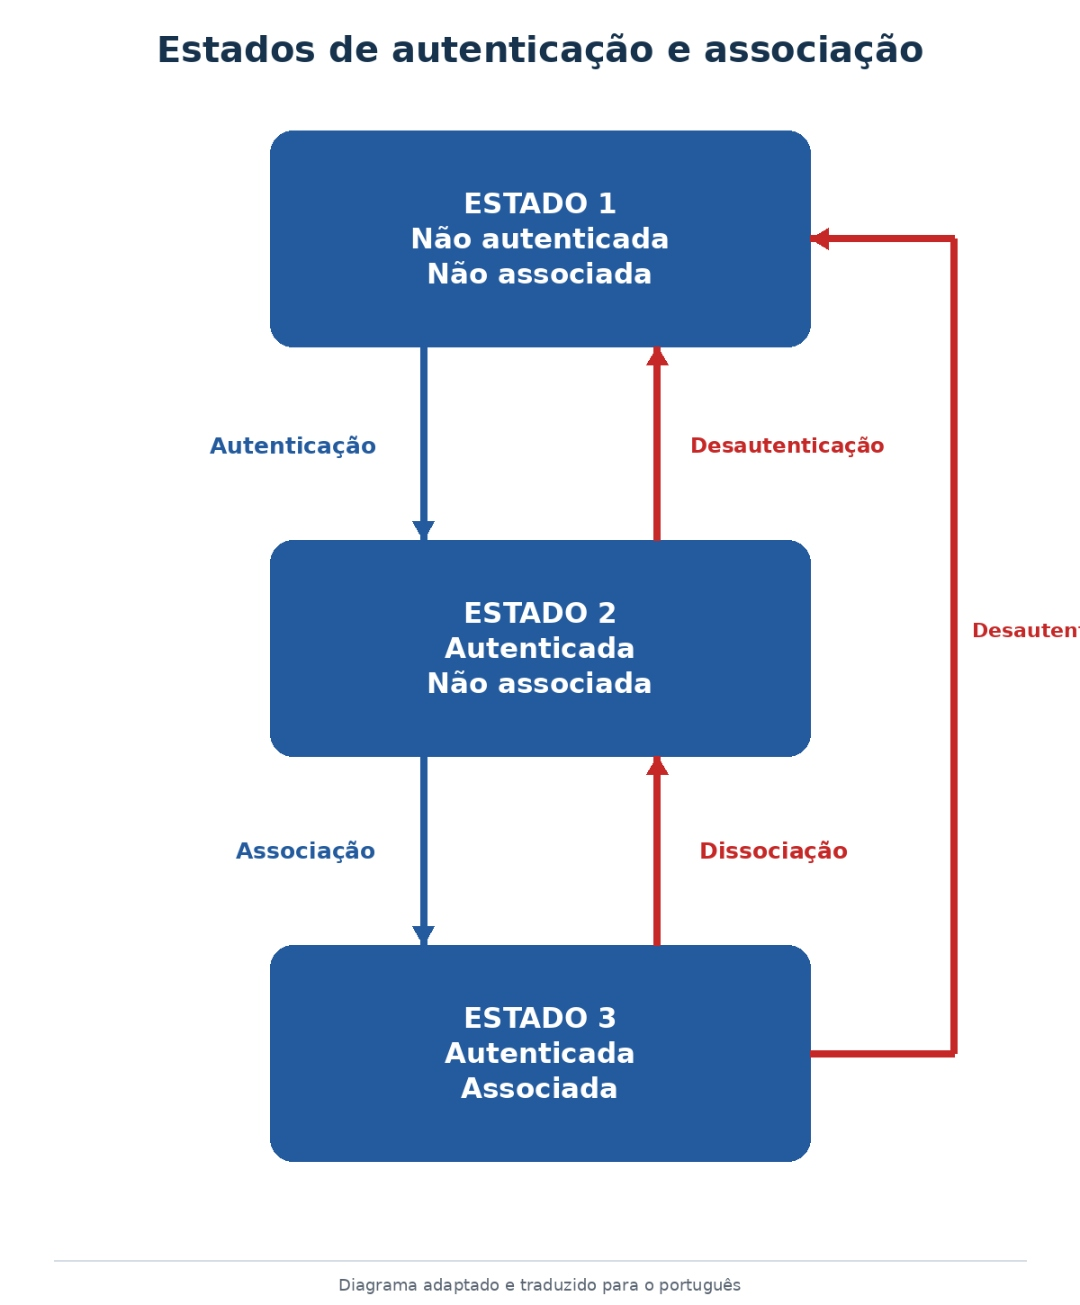
\includegraphics[width=0.53\textwidth]{estados_autenticacao}
\legend{Fonte: adaptado de Kristiyanto e Ernastuti (2020, p. 46).}
\end{figure}

\subsection{Evolução dos mecanismos de segurança: do WEP ao WPA3}

A segurança em redes IEEE 802.11 evoluiu ao longo do tempo em resposta direta à exploração das vulnerabilidades inerentes a um meio de transmissão aberto e suscetível à interceptação. O primeiro mecanismo padronizado foi o WEP (\textit{Wired Equivalent Privacy}), cujo objetivo era proporcionar um nível de confidencialidade considerado equivalente ao de redes cabeadas. O WEP baseava‑se na cifra de fluxo RC4 (\textit{Rivest Cipher 4}), associada a um código de redundância cíclica (CRC‑32) para verificação de integridade da carga útil \cite{KohliosHayajneh2018}.

A literatura, entretanto, evidencia falhas estruturais graves na concepção do WEP. O protocolo dependia de chaves estáticas, concatenadas a um vetor de inicialização (IV) de apenas 24~bits, transmitido em texto claro. Em redes com tráfego moderado ou elevado, o espaço reduzido de combinações para o IV era rapidamente esgotado, levando à sua inevitável reutilização. O reuso do IV, combinado com o fluxo de chaves gerado pelo RC4, possibilitou ataques estatísticos de criptoanálise e de recuperação passiva de chaves, permitindo que um invasor obtivesse a chave de rede em poucos minutos de tráfego capturado ou artificialmente injetado \cite{KohliosHayajneh2018,Lima2025}.

Essa experiência prática mostrou que a simples adoção de cifradores de fluxo não era suficiente para garantir confidencialidade, especialmente na ausência de um projeto cuidadoso de chaves e vetores de inicialização. A combinação de IVs curtos, chaves estáticas e reutilização de fluxos de chave tornou o WEP um mecanismo rapidamente obsoleto do ponto de vista de segurança \cite{KohliosHayajneh2018,Lima2025}. Para mitigar essas limitações sem substituir imediatamente o \textit{hardware} já instalado, a Wi‑Fi Alliance introduziu o WPA (\textit{Wi‑Fi Protected Access}) como solução transitória. O WPA passou a exigir o uso do \textit{Temporal Key Integrity Protocol} (TKIP), que modifica a forma de mistura de chaves e dos vetores de inicialização do RC4, gerando chaves dinâmicas por pacote. Além disso, incorporou um código de integridade de mensagem mais robusto, baseado no algoritmo Michael, com o objetivo de reduzir a injeção de quadros forjados e ataques de repetição \cite{KohliosHayajneh2018}.

Na sequência, o WPA2 consolidou o \textit{Advanced Encryption Standard} (AES) no modo \textit{Counter Mode with CBC-MAC Protocol} (CCMP), ou AES‑CCMP, como mecanismo padrão de proteção do tráfego de dados, elevando de forma significativa os níveis de confidencialidade e integridade em relação às versões anteriores. Apesar desses avanços, as tramas de gerenciamento permaneceram sem proteção equivalente nas redes WPA2 que não adotam PMF, de modo que, nelas, ataques de desautenticação e dissociação continuaram tecnicamente viáveis \cite{KohliosHayajneh2018}. A proteção sistemática de quadros de gestão veio com a emenda IEEE~802.11w (PMF), aplicável ao próprio WPA2, e foi reforçada pelo WPA3, que tornou o PMF obrigatório e adotou o protocolo SAE (\textit{Simultaneous Authentication of Equals}) \cite{CiscoMFP2024,EspressifWifiSecurity}.

No WPA2, o estabelecimento das chaves de sessão ocorre por meio do chamado \textit{4-way handshake}, executado após a autenticação inicial entre a estação (STA) e o ponto de acesso (AP). Nesse processo, ilustrado na Figura~\ref{fig:handshake_wpa2}, o AP envia um número aleatório (\textit{ANonce}); a STA responde com o seu próprio número (\textit{SNonce}) acompanhado de um código de integridade (MIC), o que permite a ambos derivarem a chave de sessão (\textit{Pairwise Transient Key} -- PTK); em seguida, o AP distribui a chave de grupo (\textit{Group Temporal Key} -- GTK) e a STA confirma a instalação das chaves. Somente após essa troca o tráfego de dados passa a ser cifrado com AES-CCMP \cite{KohliosHayajneh2018}. O \textit{4-way handshake}, por si só, protege os dados do usuário, mas não os quadros de gerenciamento. Quando o PMF é negociado, a terceira mensagem também entrega a IGTK, e as chaves derivadas nessa troca passam a proteger os quadros de gerenciamento robustos \cite{CiscoMFP2024}. O mesmo \textit{4-way handshake} é executado no WPA3-\textit{Personal}, como se discute a seguir.

\begin{figure}[htb]
\centering
\caption{Troca de chaves por \textit{4-way handshake} (WPA2 e WPA3-\textit{Personal})}
\label{fig:handshake_wpa2}
\begin{tikzpicture}[font=\small, >=Stealth]
\node (sta) at (0,0) {\textbf{STA (dispositivo)}};
\node (ap) at (8.5,0) {\textbf{AP (roteador)}};
\draw[thick] (0,-0.4) -- (0,-6);
\draw[thick] (8.5,-0.4) -- (8.5,-6);
\draw[->] (8.5,-1.1) -- node[above, font=\footnotesize]{1. \textit{ANonce}} (0,-1.1);
\draw[->] (0,-2.1) -- node[above, font=\footnotesize]{2. \textit{SNonce} + MIC} (8.5,-2.1);
\node[align=center, font=\footnotesize] at (4.25,-2.8) {(ambos derivam a PTK)};
\draw[->] (8.5,-3.6) -- node[above, font=\footnotesize]{3. \textit{GTK} + MIC} (0,-3.6);
\draw[->] (0,-4.6) -- node[above, font=\footnotesize]{4. Confirmação (MIC)} (8.5,-4.6);
\node[align=center, font=\footnotesize] at (4.25,-5.4) {Chaves instaladas $\rightarrow$ tráfego cifrado (AES-CCMP)};
\end{tikzpicture}
\legend{Fonte: elaborado pelo autor com base em Kohlios e Hayajneh (2018) e \citeonline{CiscoMFP2024}. A troca parte de uma PMK, derivada da senha no WPA2-PSK ou produzida pelo SAE no WPA3-\textit{Personal}. Com PMF negociado, a mensagem 3 também entrega a IGTK; sem PMF, os quadros de gerenciamento continuam desprotegidos após a troca.}
\end{figure}

O WPA3-\textit{Personal}, por sua vez, não elimina o \textit{4-way handshake}. O que o protocolo SAE (\textit{Simultaneous Authentication of Equals}), baseado em uma troca do tipo \textit{Dragonfly}, substitui é a autenticação baseada em PSK: em vez de a \textit{Pairwise Master Key} (PMK) ser derivada diretamente da senha, como no WPA2-PSK, ela é produzida por uma troca SAE realizada nos quadros de autenticação (\textit{authentication algorithm}~3), resistente a ataques de dicionário \textit{off-line}. Em seguida, o \textit{4-way handshake} é executado normalmente a partir dessa PMK para derivar as chaves de sessão \cite{KohliosHayajneh2018,EspressifWifiSecurity}. Além disso, o WPA3 torna obrigatório o PMF, que acrescenta integridade e autenticidade aos quadros de gerenciamento robustos, como os de desautenticação e dissociação, dificultando a sua falsificação. A Figura~\ref{fig:wpa3_sae_pmf} resume essas duas contribuições do WPA3 em relação às versões anteriores.

\begin{figure}[htb]
\centering
\caption{Principais contribuições de segurança do WPA3-\textit{Personal}}
\label{fig:wpa3_sae_pmf}
\resizebox{0.92\textwidth}{!}{%
\begin{tikzpicture}[font=\small, >=Stealth,
  w/.style={draw, rounded corners, minimum width=52mm, minimum height=22mm, align=center}]
\node[w, fill=blue!12, minimum width=34mm, minimum height=10mm] (root) at (0,2) {\textbf{WPA3}};
\node[w, fill=green!12] (sae) at (-3.4,-0.6) {\textbf{SAE} (\textit{Dragonfly})\\Substitui a autenticação por PSK\\e produz a PMK; resistente a\\dicionário \textit{off-line}\\(\textit{4-way handshake} mantido)};
\node[w, fill=orange!16] (pmf) at (3.4,-0.6) {\textbf{PMF} (IEEE 802.11w)\\Obrigatório no WPA3; opcional no WPA2\\Integridade e autenticidade dos\\quadros robustos (\textit{deauth} / \textit{dissoc.})\\Não garante disponibilidade};
\draw[->] (root) -- (sae);
\draw[->] (root) -- (pmf);
\end{tikzpicture}}
\legend{Fonte: elaborado pelo autor com base em Kohlios e Hayajneh (2018), \citeonline{CiscoMFP2024} e \citeonline{EspressifWifiSecurity}. O PMF impede a falsificação de quadros robustos, mas não protege contra interferência física (\textit{jamming}) nem contra outras formas de negação de serviço por rádio.}
\end{figure}

Na prática, contudo, a adoção desses mecanismos é desigual, sobretudo em ambientes compostos por dispositivos IoT de baixo custo. Muitos equipamentos legados não dispõem de recursos de \textit{hardware} ou de espaço de \textit{firmware} suficientes para suportar plenamente PMF e WPA3 \cite{Lima2025}. A permanência de dispositivos legados sem suporte a WPA3 leva, na prática, ao uso de modos de compatibilidade, como o modo de transição WPA2/WPA3. É importante notar, contudo, que a segurança não é definida para a rede como um todo: no modo de transição, o ponto de acesso anuncia mais de um conjunto de autenticação (PSK e SAE) e o PMF como opcional, como registrado nas capturas deste trabalho (Apêndice~\ref{sec:evidencias-rsn}); com o PMF opcional, estações que não suportam o IEEE~802.11w continuam autorizadas a se conectar \cite{CiscoMFP2024}, e cada estação negocia, na sua própria associação, o \textit{Authentication and Key Management} (AKM) e o uso do PMF que suporta. Assim, um dispositivo legado que negocia WPA2-PSK sem PMF permanece exposto à falsificação de quadros de gestão, sem que isso retire a proteção das estações que negociaram SAE e PMF na mesma rede. O risco do modo de transição está, portanto, na permanência de associações desprotegidas, e não em um rebaixamento automático de todas as estações, o que é especialmente relevante em redes residenciais com muitos dispositivos IoT de baixo custo \cite{Hassija2019,Lima2025}. Os resultados deste trabalho ilustram essa negociação por associação (Seção~\ref{subsec:consolidacao_resultados}).

Em síntese, a evolução do IEEE 802.11 demonstra um avanço consistente nos mecanismos de proteção do tráfego de dados, mas revela também uma defasagem histórica na proteção das tramas de gerenciamento. Essa assimetria cria uma superfície de ataque particularmente sensível: nas associações que não negociam PMF, quadros de desautenticação e dissociação podem ser forjados e injetados no meio por qualquer dispositivo com capacidade de transmissão em nível MAC. No contexto deste trabalho, essa característica é explorada experimentalmente por meio de microcontroladores de baixo custo, que atuam como vetores de ataque contra dispositivos IoT em cenários residenciais.

A evolução dos mecanismos de segurança é apresentada na Figura~\ref{fig:evolucao_seguranca_80211}. O diagrama relaciona WEP, WPA, WPA2, IEEE~802.11w e WPA3, destacando o fortalecimento progressivo da proteção dos dados e, posteriormente, dos quadros de gerenciamento \cite{Hiertz2010,KohliosHayajneh2018,CiscoMFP2024}. A sequência não deve ser lida como uma separação rígida entre WPA2 desprotegido e WPA3 protegido: o PMF do IEEE~802.11w pode ser usado com WPA2, é obrigatório no WPA3 e, em ambos os casos, é negociado em cada associação \cite{CiscoMFP2024}.

\begin{figure}[htb]
\centering
\caption{Evolução dos mecanismos de segurança no padrão IEEE 802.11}
\label{fig:evolucao_seguranca_80211}
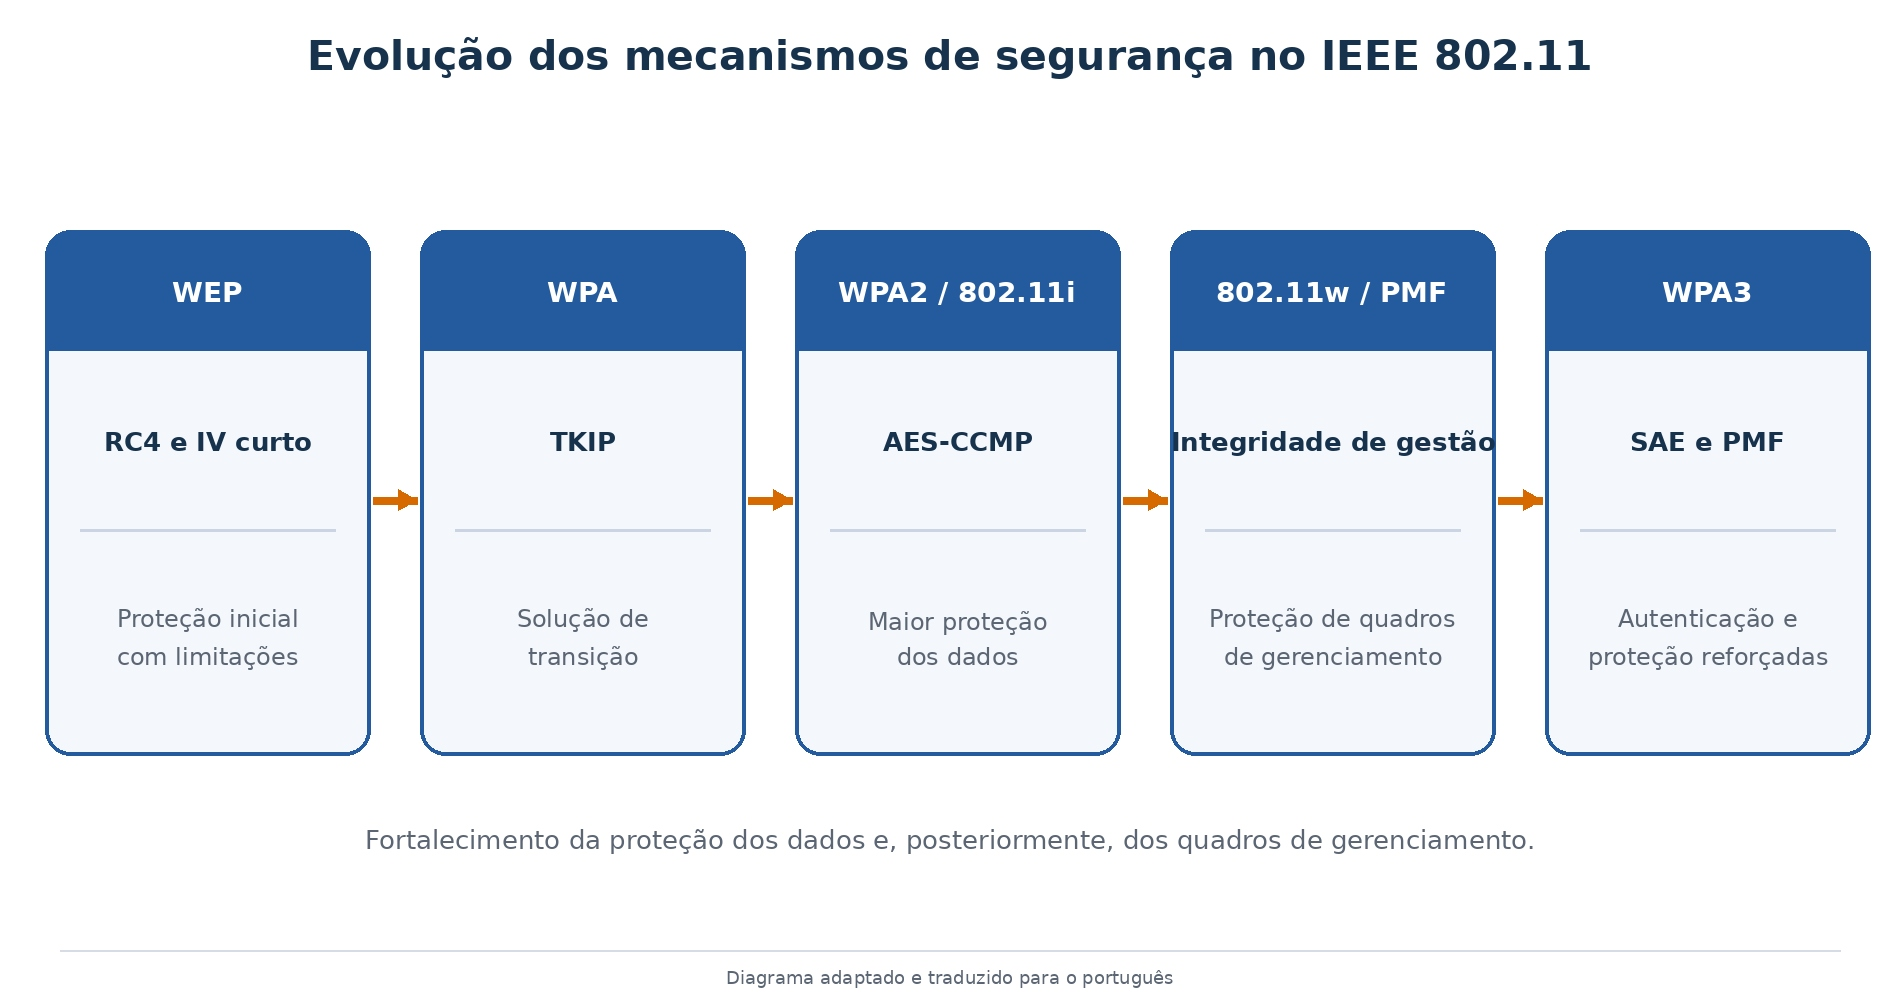
\includegraphics[width=0.98\textwidth]{evolucao_seguranca_80211}
\legend{Fonte: elaborado pelo autor com base em Hiertz et al. (2010), para WEP, WPA e WPA2, e em \citeonline{KohliosHayajneh2018} e \citeonline{CiscoMFP2024}, para 802.11w e WPA3. O IEEE~802.11w (PMF) é opcional no WPA2 e obrigatório no WPA3; protege apenas quadros de gerenciamento robustos e só vale para as associações que o negociam.}
\end{figure}

\section{Microcontroladores e hardware ofensivo de baixo custo}

\subsection{Arquitetura de hardware das plataformas ESP8266, ESP32 e ESP32-S3}

O barateamento e a miniaturização de componentes semicondutores deram origem a sistemas em chip (SoC) com alta capacidade de processamento e conectividade, que atualmente constituem parte essencial da indústria de IoT. Nesse contexto, as plataformas fabricadas pela Espressif Systems, notadamente o ESP8266, o ESP32 e o ESP32-S3, destacam-se pela relação custo-benefício e pela ampla adoção em projetos comerciais e acadêmicos.

\citeonline{LitayemAlsadi2023} exploram em detalhe a arquitetura dessas plataformas. O ESP8266 é baseado no microprocessador L106, de 32~bits da Tensilica, operando tipicamente a 80~MHz, com cerca de 160~kB de \textit{Static Random-Access Memory} (SRAM) e integração nativa do protocolo IEEE~802.11 b/g/n, suportando integralmente a pilha \textit{Transmission Control Protocol}/\textit{Internet Protocol} (TCP/IP). Essa integração elimina a necessidade de \textit{chipsets} adicionais para conectividade Wi-Fi, reduzindo custos e complexidade de projeto. O ESP32 representa um salto arquitetural significativo: incorpora processador Xtensa Dual-Core LX6 de 32~bits, SRAM expandida para aproximadamente 520~kB, além de módulos combinados de Wi‑Fi e Bluetooth, tanto em modo clássico quanto em \textit{Low Energy} \cite{LitayemAlsadi2023}.

O ESP32-S3, utilizado neste trabalho por meio da placa LILYGO T-Embed CC1101 Plus, não deve ser confundido com o ESP32 original. Trata-se de um SoC posterior, com processador Xtensa LX7 de 32~bits e dois núcleos, de até 240~MHz, 512~kB de SRAM, Wi-Fi IEEE~802.11 b/g/n restrito à faixa de 2,4~GHz (canais de 20 e 40~MHz) e Bluetooth \textit{Low Energy} 5, sem o Bluetooth clássico do ESP32 \cite{EspressifS3Datasheet}. Em todos esses casos, trata-se de SoCs com rádio 802.11 embutido, capazes de executar aplicações e controlar diretamente a interface sem fio.

A facilidade de programação desses microcontroladores, suportada por ambientes como Arduino IDE, PlatformIO e MicroPython, somada à capacidade de realizar atualizações \textit{Over-The-Air} (OTA), tornou essas plataformas particularmente adequadas para o desenvolvimento rápido de aplicações conectadas. Do ponto de vista da engenharia de segurança, o mesmo conjunto de características — baixo custo, alta disponibilidade e acesso direto ao transceptor Wi‑Fi — favorece seu emprego em experimentos de segurança ofensiva, notadamente em cenários de testes de intrusão em redes IEEE~802.11 e em estudos sobre a exploração de vulnerabilidades em tramas de gerenciamento.

\subsection{Modos de operação: modo estação, \textit{access point} e modo monitor}

As plataformas ESP possuem uma pilha de rádio flexível, capaz de operar em múltiplos estados lógicos, o que permite contornar parte das camadas tradicionais de rede \cite{LitayemAlsadi2023}. Os modos operacionais padrão incluem o modo estação (STA), no qual o microcontrolador atua como cliente conectando-se a um roteador Wi‑Fi existente, e o modo \textit{Access Point} (AP), em que o próprio chip passa a atuar como ponto de acesso, fornecendo endereços IP e hospedando uma rede local. Esse último modo é também explorado em cenários de \textit{Evil Twin}, nos quais um AP falso imita o identificador de serviço (SSID) e outros parâmetros do roteador legítimo, com as restrições discutidas na Seção~\ref{subsec:evil_twin}.

Para fins de auditoria de segurança, destaca-se a captura de quadros do canal, que exige distinguir dois conceitos frequentemente confundidos. No modo promíscuo, a interface, associada a uma rede, deixa de descartar os quadros daquela rede que não são destinados ao seu endereço MAC e os repassa ao sistema. No modo monitor, a interface não precisa estar associada: ela entrega todos os quadros IEEE~802.11 recebidos no canal sintonizado, inclusive quadros de gerenciamento e de controle e quadros de outras redes, com o cabeçalho 802.11 original. Para a análise de quadros de desautenticação e de associação, o modo relevante é o monitor, empregado neste trabalho com o adaptador AR9271. Nos chips da Espressif, essa função é oferecida pelo próprio \textit{framework} oficial como modo \textit{sniffer}, que, apesar de ser ativado por uma função chamada \texttt{esp\_wifi\_set\_promiscuous}, entrega quadros de gerenciamento, de dados e de controle e pode operar sem associação \cite{EspressifWifiModes}. Essa funcionalidade concede ao dispositivo a capacidade de atuar como um \textit{sniffer} de pacotes, extraindo cabeçalhos de comunicação da vizinhança sem fio \cite{Lima2025}. Na prática, isso permite identificar BSSIDs, endereços MAC de estações, tipos de quadros de gerenciamento e parâmetros de configuração de redes alvo, insumos essenciais para a construção de ataques de desautenticação direcionados.

\subsection{Injeção de pacotes e \textit{bypassing} de protocolos via hardware programável}

A capacidade de injeção de pacotes (\textit{packet injection}) representa o complemento ofensivo do modo monitor. Enquanto o modo monitor permite apenas a escuta passiva do meio, a injeção torna possível construir arbitrariamente sequências de bytes na memória do microcontrolador e transmiti-las diretamente pelo ar, ignorando parte do controle de estado normalmente imposto pela pilha de rede do sistema operacional. Em outras palavras, o microcontrolador deixa de seguir o fluxo convencional de associação, autenticação e estabelecimento de sessão, passando a emitir quadros IEEE~802.11 “sob medida” em nível MAC.

Ferramentas de código aberto, como o projeto \textit{esp8266\_deauther}, empacotam essas instruções de baixo nível em bibliotecas de uso relativamente simples. \citeonline{LitayemAlsadi2023} destacam que essas aplicações, muitas vezes disponibilizadas em repositórios públicos, transformam um chip de custo extremamente reduzido em um vetor de ataque efetivo. Ao manipular diretamente a interface de programação de aplicações do módulo Wi‑Fi da Espressif, o \textit{software} contorna validações usuais, construindo tramas de desautenticação a partir de endereços MAC obtidos previamente em captura de tráfego e efetivando, contra estações que não negociaram PMF, ataques de negação de serviço sem necessidade de \textit{hardware} profissional dedicado. Assim, funções originalmente concebidas para testes de laboratório ou desenvolvimento acabam sendo reutilizadas em contextos ofensivos, democratizando o acesso a técnicas antes restritas a equipamentos especializados.

\subsection{Ferramentas portáteis e a democratização do \textit{pentesting}}

O \textit{pentesting} sem fio, antes associado a \textit{notebooks} com distribuições Linux e adaptadores específicos, passou a contar com dispositivos portáteis de baixo custo. O Flipper Zero é um exemplo conhecido: reúne funções em Sub-1~GHz, \textit{Radio-Frequency Identification} (RFID), \textit{Near-Field Communication} (NFC) e infravermelho e, para Wi-Fi, depende de módulos externos baseados em ESP8266 ou ESP32, que realizam varreduras e ataques de desautenticação sem computador auxiliar \cite{James2023}. Esse trabalho é um \textit{preprint} que, segundo o próprio documento, não passou por revisão por pares; por isso, é usado aqui apenas para descrever a categoria da plataforma, e não como evidência de desempenho. A plataforma usada neste trabalho, a LILYGO T-Embed CC1101 Plus com \textit{firmware} Bruce, segue a mesma lógica, mas integra o ESP32-S3 na própria placa. Essa portabilidade indica que dispositivos da família ESP são, ao mesmo tempo, representativos do desenvolvimento IoT e instrumentos viáveis para ensaios de desautenticação em laboratório \cite{LitayemAlsadi2023}.

\section{Internet das Coisas e vulnerabilidades de borda}

\subsection{Definições e arquiteturas de redes de sensores}

O termo Internet das Coisas refere-se à rede global de dispositivos físicos incorporados a eletrônica, \textit{software} e sensores, que lhes conferem a capacidade de adquirir, processar e transferir dados sobre o ambiente e sobre sua própria operação. \citeonline{LiXuZhao2015} descrevem a arquitetura clássica da IoT como um modelo estratificado em três camadas principais: camada de percepção, camada de rede e camada de aplicação.

A camada de percepção é composta por nós terminais, como câmeras, sensores de temperatura, atuadores e etiquetas RFID, responsáveis por interagir com o mundo físico e digitalizar sinais. A camada de rede reúne a infraestrutura encarregada do roteamento e da transmissão dos dados capturados, incluindo roteadores Wi‑Fi, \textit{gateways} Zigbee e outros dispositivos de interconexão. Já a camada de aplicação corresponde à interface com o usuário e aos sistemas em nuvem responsáveis pelo processamento, armazenamento e análise das informações em larga escala \cite{LiXuZhao2015}.

No contexto da IoT de consumo, a camada de rede depende de forma destacada do protocolo IEEE~802.11, sobretudo pela ampla presença de roteadores Wi‑Fi domésticos. Essa dependência transforma as vulnerabilidades históricas do padrão em ameaças diretas à integridade da própria camada de percepção, uma vez que a interrupção da conectividade compromete imediatamente o funcionamento de sensores, câmeras, lâmpadas e demais dispositivos conectados. Assim, fragilidades na comunicação sem fio assumem impacto direto sobre a disponibilidade de serviços automatizados em ambientes residenciais e corporativos, aproximando vulnerabilidades de camada de enlace de consequências perceptíveis ao usuário final.

A organização desses elementos em quatro níveis é apresentada na Figura~\ref{fig:arquitetura_camadas_iot}. A camada de percepção reúne sensores, atuadores e dispositivos responsáveis pela interação com o ambiente; a camada de rede transporta os dados; o \textit{middleware} oferece processamento, armazenamento e serviços intermediários; e a camada de aplicação disponibiliza as funcionalidades ao usuário. Os \textit{gateways} realizam a integração entre dispositivos, redes e protocolos heterogêneos \cite{Hassija2019}.

\begin{figure}[htb]
\centering
\caption{Arquitetura em camadas de um sistema IoT}
\label{fig:arquitetura_camadas_iot}
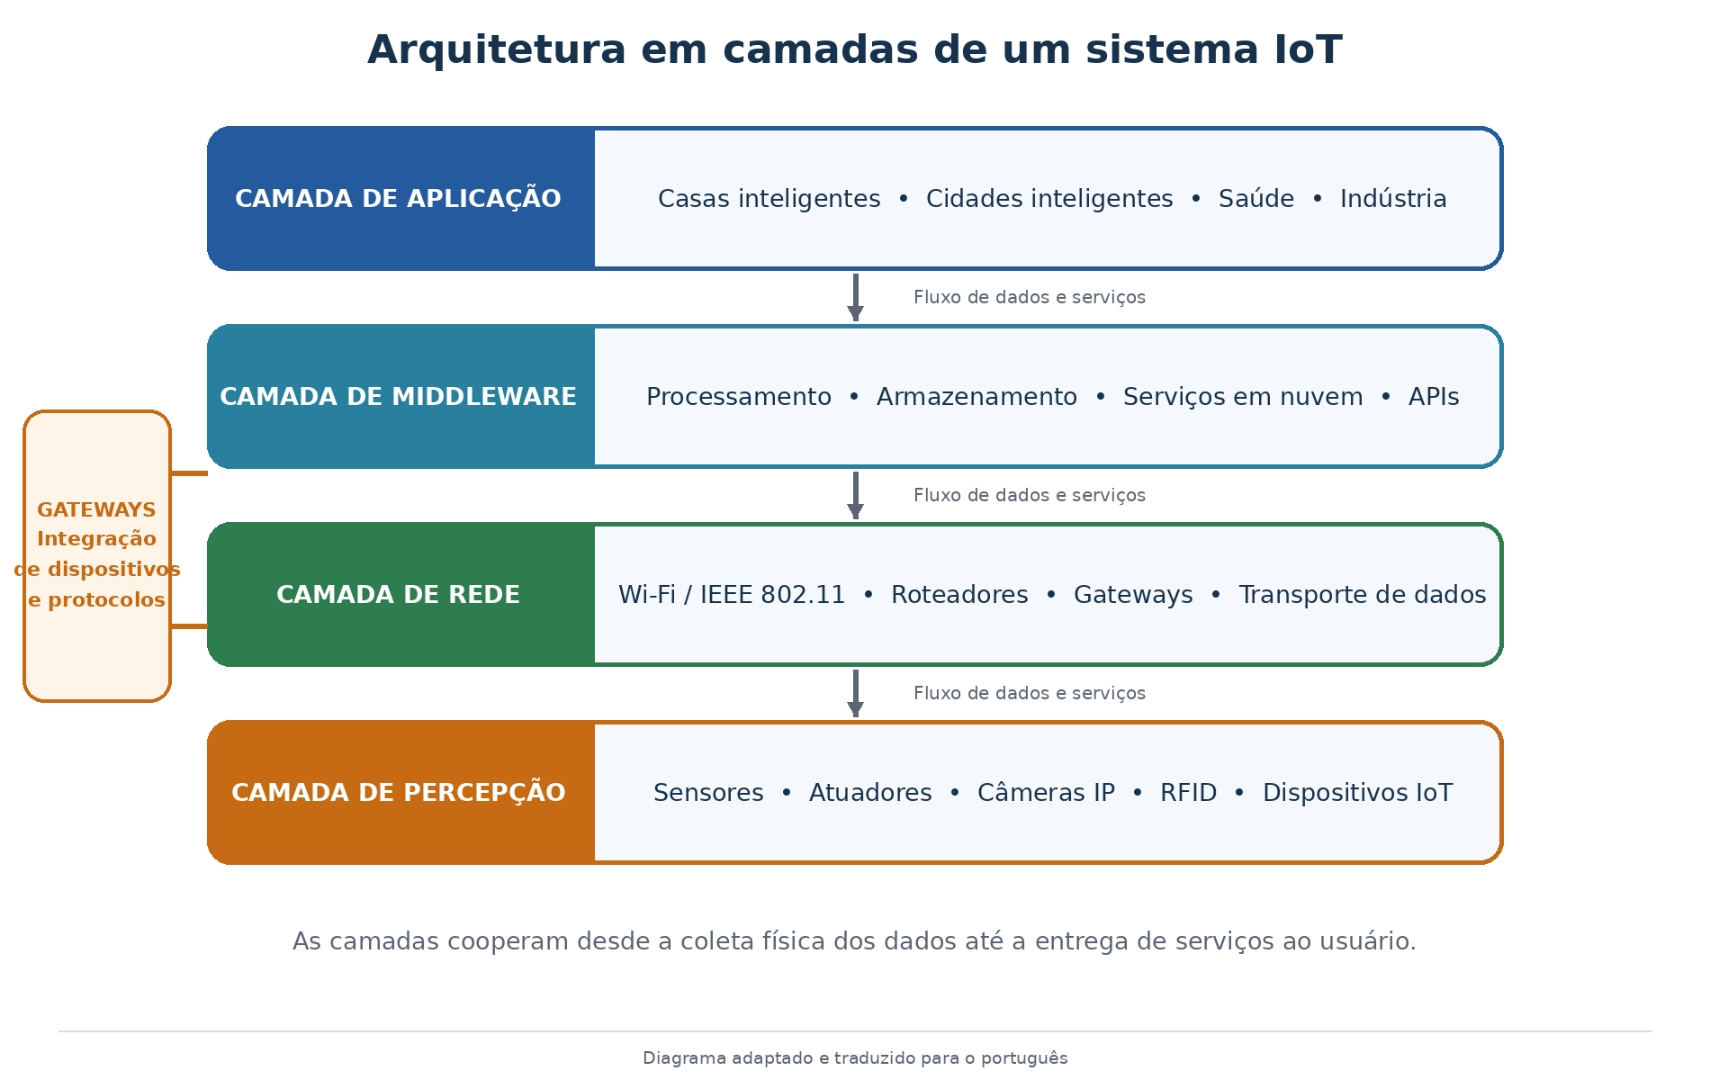
\includegraphics[width=0.98\textwidth]{arquitetura_camadas_iot}
\legend{Fonte: adaptado de Hassija et al. (2019).}
\end{figure}

\subsection{Restrições de hardware e energia}

Para garantir viabilidade comercial, fabricantes de dispositivos IoT frequentemente utilizam processadores de baixa potência, memória restrita e módulos de comunicação simplificados, e muitos equipamentos operam sob limites energéticos severos, empregando técnicas como o \textit{Target Wake Time} (TWT) para permanecer longos períodos em suspensão \cite{FarhadPyun2022}. \citeonline{Yuksel2020} analisou o consumo de energia de um dispositivo IoT baseado em Wi-Fi e a influência do módulo Wi-Fi nesse consumo, sem tratar de ataques. A partir disso, formula-se apenas como hipótese que, sob um ataque contínuo de desautenticação, um dispositivo nessas condições seja forçado a despertar repetidamente para renegociar a associação, elevando o consumo além de ficar indisponível. Essa hipótese não foi testada: o consumo energético não foi medido neste trabalho, cujos dispositivos avaliados são alimentados pela rede elétrica, à exceção do \textit{smartphone}.

\subsection{Atualização de \textit{firmware} e suporte a WPA3 e PMF}

A correção para a fragilidade das tramas de gerenciamento passa pelo uso de PMF, seja com WPA2, seja com WPA3. \citeonline{Lima2025} observa que uma parcela expressiva dos dispositivos inteligentes comercializados, como lâmpadas, interruptores e sensores de presença, utiliza módulos de rádio limitados ao Wi-Fi~4 (IEEE~802.11n), operando apenas na faixa de 2,4~GHz. Essa característica, porém, não impede por si só o uso de WPA3 ou de PMF, pois ambos são mecanismos de segurança da camada MAC, independentes da geração da camada física e da faixa de frequência. O próprio ESP32-S3 é um contraexemplo: seu rádio é IEEE~802.11 b/g/n e opera somente em 2,4~GHz \cite{EspressifS3Datasheet}, e ainda assim a pilha oficial da Espressif oferece suporte a WPA3-\textit{Personal} e a PMF nos modos opcional e obrigatório \cite{EspressifWifiSecurity}. Nos ensaios deste trabalho, a lâmpada inteligente, que também opera em 2,4~GHz, negociou SAE com PMF obrigatório (Apêndice~\ref{sec:evidencias-rsn}).

A barreira, portanto, está menos no rádio e mais no \textit{software}: módulos com \textit{drivers} gravados em \textit{Read-Only Memory} (ROM), pouco espaço para atualizações ou fabricantes que não distribuem novas versões de \textit{firmware} podem deixar de oferecer SAE e PMF mesmo quando o \textit{hardware} os comportaria \cite{Lima2025}. Para preservar a compatibilidade com esses dispositivos, o roteador pode ser configurado em modo de transição WPA2/WPA3, como no cenário misto deste trabalho. Como a negociação ocorre por associação (Seção~\ref{subsec:consolidacao_resultados}), essa escolha não rebaixa a segurança das estações que suportam SAE e PMF, mas mantém expostas à desautenticação forjada as estações que negociam WPA2 sem PMF \cite{Lima2025}.

\subsection{Taxonomia de ameaças em dispositivos de consumo}

O impacto das restrições de \textit{hardware} resulta em um ecossistema frágil sob múltiplas perspectivas. \citeonline{Hassija2019} apresentam uma taxonomia abrangente de ameaças voltada especificamente para a IoT, mapeando vetores de ataque em diferentes camadas da arquitetura. Entre esses vetores, destacam-se ataques de rádio e enlace, como \textit{jamming}, falsificação de identidade, negação de serviço, exploração de mecanismos de autenticação deficientes e interceptação de tráfego \cite{Hassija2019}.

Três conceitos dessa taxonomia precisam ser distinguidos, pois são frequentemente tratados como sinônimos. A \textbf{falsificação de quadros de desautenticação} é um ataque de protocolo: o atacante transmite quadros de gerenciamento válidos em formato, mas com endereço de origem forjado, e só é efetivo contra associações que não negociaram PMF. Na prática, o atacante se passa pelo ponto de acesso: o quadro é enviado com o endereço MAC do ponto de acesso (BSSID) como origem e o endereço da estação-alvo como destino, ou o endereço de difusão, para atingir todas as estações da rede. Como, sem PMF, a estação não tem meios de verificar a autenticidade do quadro, ela o aceita como se tivesse sido enviado pelo próprio ponto de acesso e encerra a associação \cite{KohliosHayajneh2018}. A \textbf{negação de serviço} não é uma técnica, mas uma categoria de efeito, a perda de disponibilidade, que pode ser obtida por diversos meios, entre eles a falsificação de quadros. O \textbf{\textit{jamming}}, por fim, é interferência na camada física: o atacante ocupa ou corrompe o canal de rádio, independentemente do conteúdo dos quadros \cite{Hassija2019,Amoordon2022}. O PMF atua apenas sobre o primeiro caso: garante a integridade e a autenticidade dos quadros de gerenciamento robustos \cite{CiscoMFP2024}, mas não garante disponibilidade. Interferência física, ocupação do canal por grande volume de quadros e ataques a quadros que o PMF não protege, como \textit{beacons}, autenticação e associação, permanecem possíveis mesmo com PMF ativo.

Em ambientes conectados por Wi-Fi, essas ameaças exploram diretamente a dependência da comunicação sem fio. Em vez de comprometer o sigilo dos dados por meio de quebra criptográfica, muitos ataques exploram a lógica de controle e coordenação da rede, impondo indisponibilidade, perda de sincronização e reconexões sucessivas. Em redes IoT de consumo, tais efeitos se traduzem em dispositivos que deixam de atuar conforme o esperado e em perdas de monitoramento em tempo real.

À luz dessa taxonomia, o ataque investigado neste trabalho é a falsificação de quadros de desautenticação, cujo efeito pretendido é a negação de serviço na camada de enlace; ele não envolve \textit{jamming}. Sua particularidade é atingir o elo de borda entre a camada de rede (roteadores Wi-Fi) e a camada de percepção (dispositivos IoT). É a interseção entre limitações de \textit{firmware}, dependência do IEEE~802.11 e associações sem PMF que torna o cenário investigado sensível a ataques simples, porém de alto impacto prático.

A Figura~\ref{fig:taxonomia_ameacas_iot} sintetiza as principais ameaças associadas às camadas de percepção, rede, \textit{middleware} e aplicação. Para este estudo, destacam-se os ataques de interferência e privação de sono na camada de percepção, bem como os ataques de negação de serviço e aos dados em trânsito na camada de rede, pois esses vetores podem comprometer a disponibilidade dos dispositivos conectados por IEEE~802.11 \cite{Hassija2019}.

\begin{figure}[htb]
\centering
\caption{Taxonomia de ameaças de segurança por camada da IoT}
\label{fig:taxonomia_ameacas_iot}
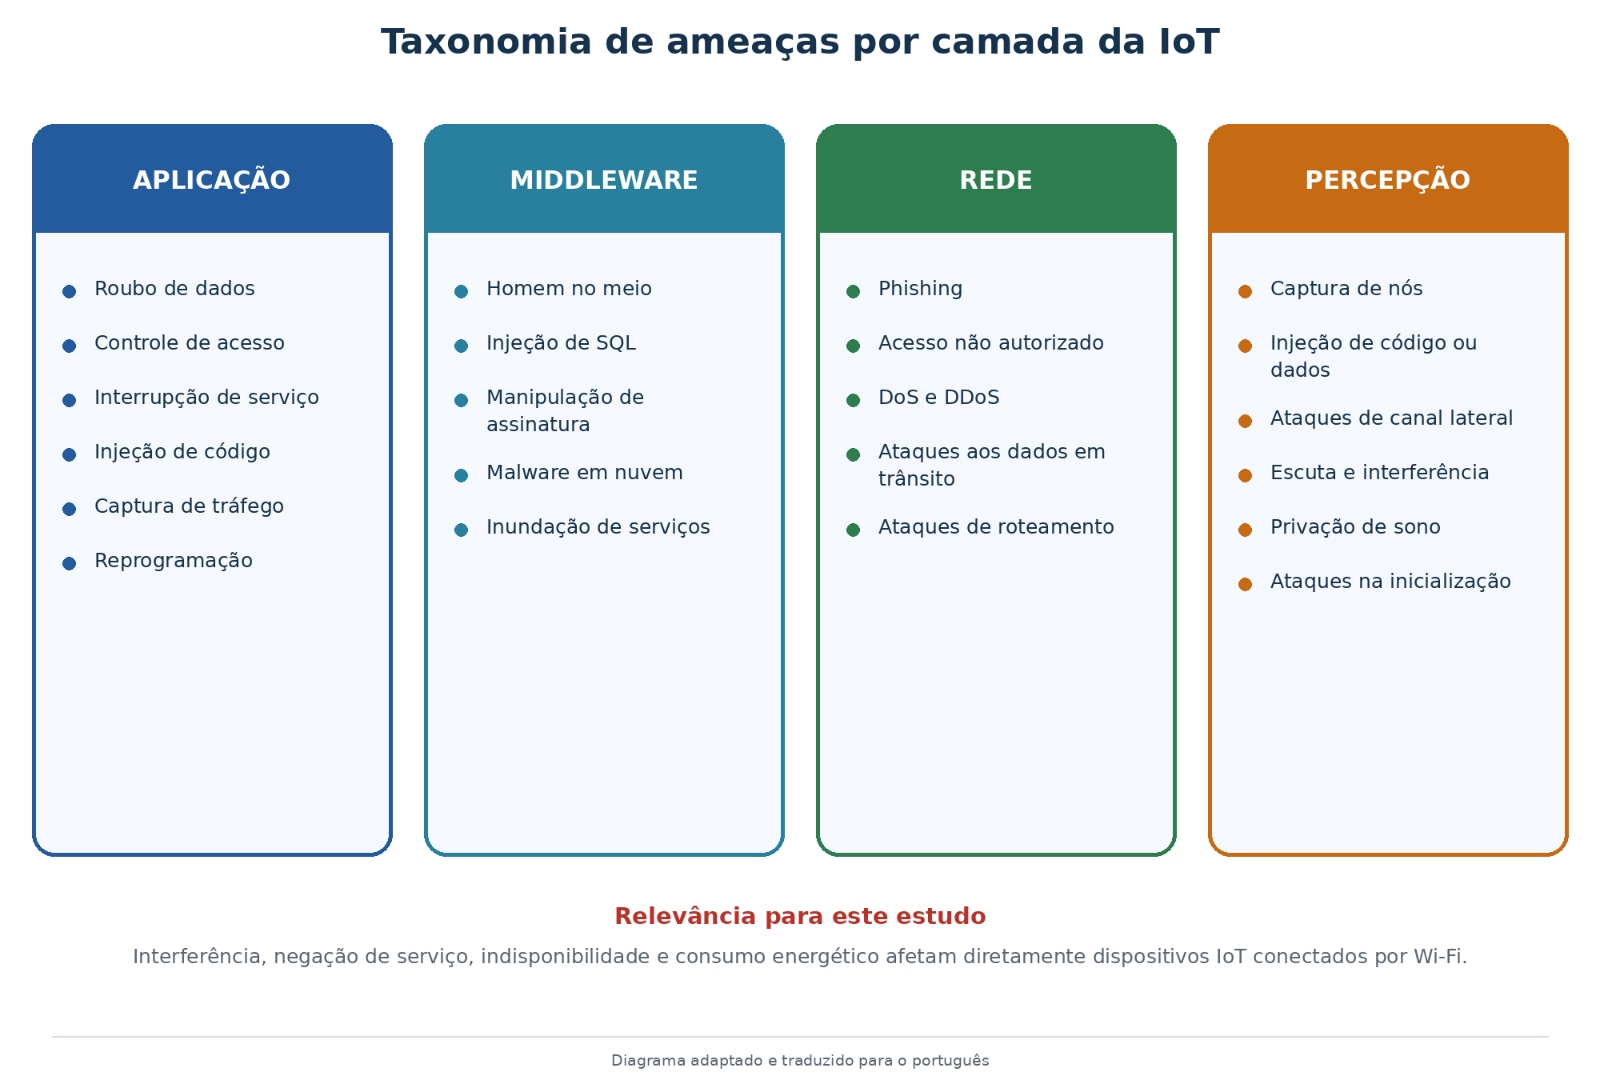
\includegraphics[width=0.98\textwidth]{taxonomia_ameacas_iot}
\legend{Fonte: adaptado de Hassija et al. (2019).}
\end{figure}

\section{Avaliação prática e estado da arte}

\subsection{Ataques combinados: desautenticação e \textit{Evil Twin}}
\label{subsec:evil_twin}

O ataque de desautenticação também é citado como etapa preparatória de intrusões mais sofisticadas, como o \textit{Evil Twin}. \citeonline{Amoordon2022} documentam a ocorrência combinada da criação de pontos de acesso falsos, \textit{jamming} de varredura de frequência e ataques de desautenticação em redes IEEE~802.11.

Nesse ataque, o atacante configura um ponto de acesso falso que replica informações do roteador legítimo, como SSID, BSSID e canal, eventualmente com potência maior, e envia quadros de desautenticação para que a vítima perca a conexão e procure novamente a rede \cite{LitayemAlsadi2023,Amoordon2022}. Copiar o SSID e aumentar a potência, contudo, não garante que o cliente se autentique no clone quando a rede legítima é protegida. No WPA2-PSK, o \textit{4-way handshake} exige que os dois lados demonstrem conhecer a senha: a mensagem~3 do ponto de acesso carrega um MIC calculado com a chave derivada dela, e um ponto de acesso que não a conhece não completa a troca; no WPA3-\textit{Personal}, a troca SAE tem o mesmo efeito \cite{KohliosHayajneh2018}. Assim, a reconexão automática a um clone só se completa se o atacante já conhecer a senha ou se o dispositivo aceitar uma rede com o mesmo nome e segurança diferente (por exemplo, aberta), comportamento que depende da implementação de cada cliente.

Por isso, dois cenários devem ser separados. No primeiro, a \textbf{reconexão automática de um dispositivo IoT}, não há interação humana: sem a senha, o clone não conclui a associação, e o efeito prático do ataque tende a se limitar à indisponibilidade. No segundo, um \textbf{usuário interage com um portal falso}: o atacante oferece uma rede aberta com nome semelhante e um portal cativo que simula a interface do roteador, e a pessoa, motivada pela queda da conexão, é persuadida a digitar a senha da rede \cite{YeboahOforiHawsh2023}. Esse segundo cenário depende de engenharia social, e não de uma falha de autenticação do protocolo, e não se aplica diretamente a dispositivos IoT sem interface para digitar credenciais. Neste trabalho, apenas a etapa de desautenticação foi avaliada.

O encadeamento entre a desautenticação e a criação de um ponto de acesso malicioso é representado na Figura~\ref{fig:ataque_evil_twin}, que deve ser lida com as condições descritas acima.

\begin{figure}[htb]
\centering
\caption{Funcionamento conceitual de um ataque Evil Twin em uma rede sem fio}
\label{fig:ataque_evil_twin}
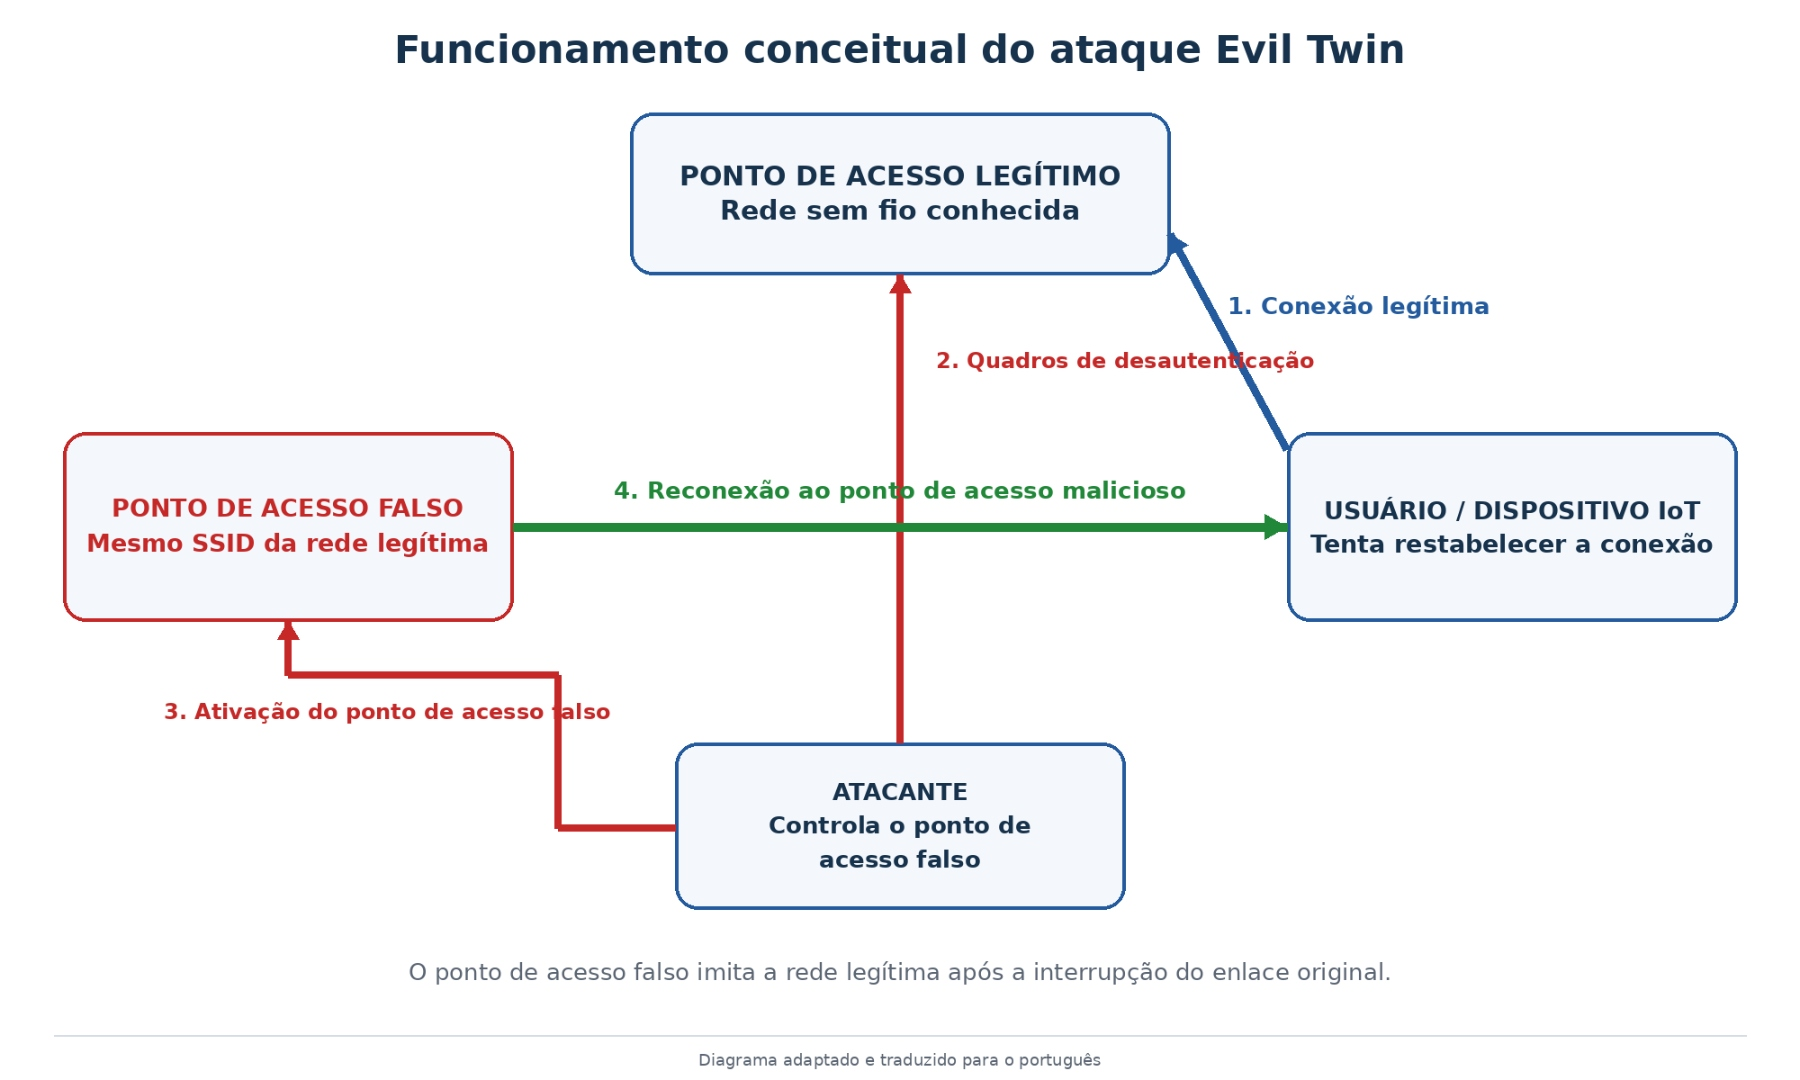
\includegraphics[width=0.98\textwidth]{ataque_evil_twin}
\legend{Fonte: adaptado de Yeboah-Ofori e Hawsh (2023). A captura da vítima pelo ponto de acesso falso pressupõe que o atacante conheça a senha da rede ou que a vítima aceite uma rede aberta e interaja com o portal falso; a cópia do SSID e o aumento de potência não bastam em redes WPA2-PSK ou WPA3-SAE.}
\end{figure}

\subsection{Análise de impacto: o estudo de Kristiyanto e Ernastuti}

\citeonline{KristiyantoErnastuti2020} realizaram um teste de penetração externa utilizando o microcontrolador NodeMCU ESP8266 para atacar a conectividade de uma câmera IP com um roteador Wi-Fi. Para quantificar o impacto, os autores utilizaram \textit{softwares} do tipo \textit{sniffer}, como o CommView, capazes de registrar o tráfego no ar.

A análise demonstrou degradações imediatas na qualidade da rede. Ao ser alvejada por pacotes de desautenticação, a câmera IP perdeu o sinal de vídeo, e os registros técnicos indicaram que o dispositivo tentou mitigar a interferência por meio de saltos de canal. Além disso, os dados de telemetria mostraram queda da taxa de transferência de dados do ambiente e anomalias em elementos de controle da comunicação, como os \textit{retry bits} e o \textit{sequence number}, que sofreram reinicializações inesperadas durante a troca de dados \cite{KristiyantoErnastuti2020}. Esse resultado é coerente com a premissa de que proteger apenas os dados do usuário, sem proteger os quadros de gerenciamento, mantém a disponibilidade dos dispositivos exposta \cite{Lima2025}.

A topologia utilizada por Kristiyanto e Ernastuti (2020) é apresentada na Figura~\ref{fig:topologia_deauth_esp8266}. O cenário reúne um ESP8266 como plataforma de teste, um ponto de acesso e uma câmera IP como dispositivo IoT avaliado, constituindo uma referência experimental diretamente relacionada ao recorte deste trabalho.

\begin{figure}[htb]
\centering
\caption{Topologia experimental de um ataque de desautenticação com ESP8266}
\label{fig:topologia_deauth_esp8266}
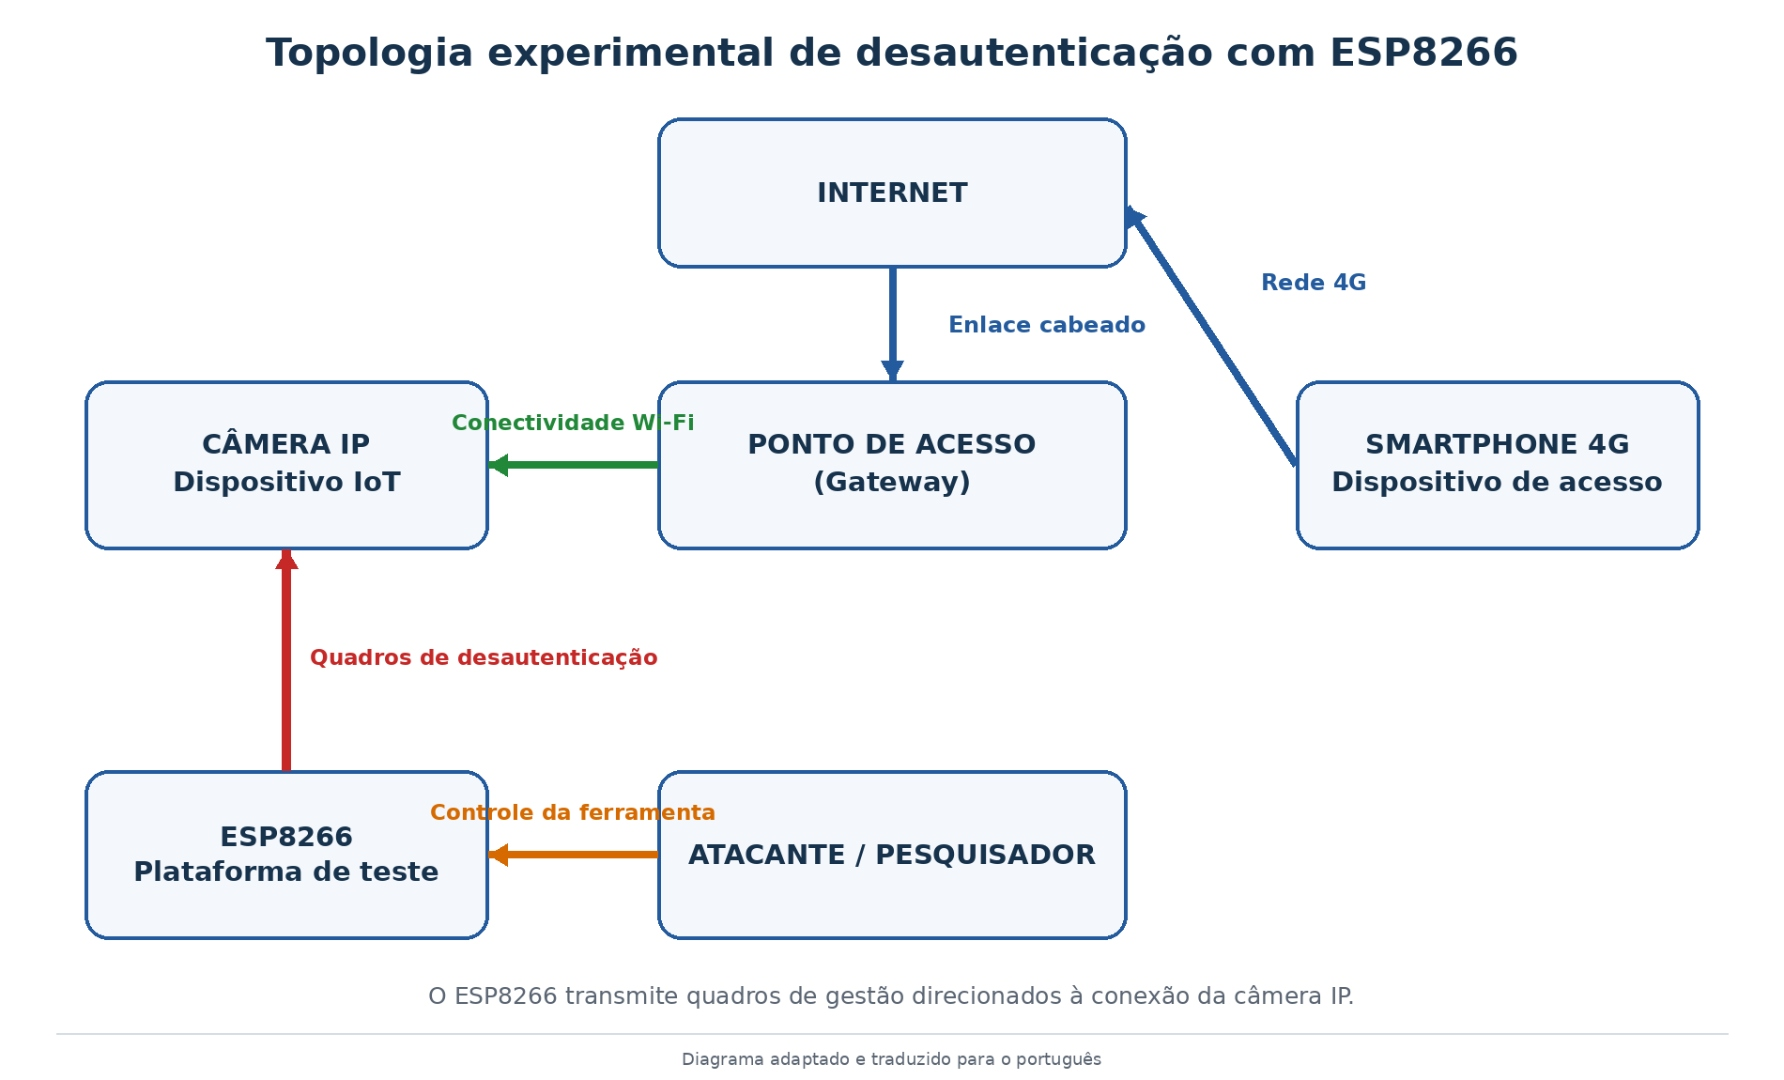
\includegraphics[width=0.94\textwidth]{topologia_deauth_esp8266}
\legend{Fonte: adaptado de Kristiyanto e Ernastuti (2020, p. 48).}
\end{figure}

\section{Trabalhos relacionados}
\label{sec:trabalhos_relacionados}

Esta seção compara este trabalho com os estudos mais próximos do seu recorte. O Quadro~\ref{quad:trabalhos-relacionados} organiza, para cada estudo, o equipamento de ataque ou análise, os dispositivos avaliados, a condição de segurança e de PMF, as métricas, o número de repetições, as limitações e a diferença em relação a este trabalho. Quando o texto original não informa um item, a célula indica ``Não informado''; nenhuma informação foi estimada.

\begin{landscape}
\begin{quadro}[p]
\centering
\caption{Comparação entre trabalhos relacionados e este estudo}
\label{quad:trabalhos-relacionados}
\marcadoresTabela
\scriptsize
\setlength{\tabcolsep}{2.5pt}
\renewcommand{\arraystretch}{1.15}
\begin{tabular}{|>{\raggedright\arraybackslash}p{2.2cm}|>{\raggedright\arraybackslash}p{2.7cm}|>{\raggedright\arraybackslash}p{2.6cm}|>{\raggedright\arraybackslash}p{2.9cm}|>{\raggedright\arraybackslash}p{2.9cm}|>{\raggedright\arraybackslash}p{2.0cm}|>{\raggedright\arraybackslash}p{2.6cm}|>{\raggedright\arraybackslash}p{3.4cm}|}
\hline
\textbf{Autor/ano} & \textbf{Equipamento} & \textbf{Dispositivos} & \textbf{Segurança/PMF} & \textbf{Métricas} & \textbf{Repetições} & \textbf{Limitações} & \textbf{Diferença para este TCC} \\ \hline
\citeonline{KristiyantoErnastuti2020} & NodeMCU ESP8266 (ataque); CommView (captura) & Câmera IP e roteador Wi-Fi & Não informado no texto; o artigo afirma que os quadros de gerenciamento não são criptografados & Perda do vídeo, vazão, \textit{retry bits}, \textit{sequence number}, saltos de canal & Não informado (um cenário descrito) & Um único tipo de dispositivo (câmera IP) & Quatro dispositivos, dois cenários de segurança, AKM e PMF verificados por associação, tempo sem resposta medido por \textit{ping} \\ \hline
\citeonline{Amoordon2022} & \textit{aireplay-ng} (desautenticação); \textit{hostapd} (AP falso); Matlab e gerador de sinal (\textit{jamming}); captura em modo monitor & Computador portátil (cliente) e \textit{Raspberry Pi} (servidor), sem dispositivos IoT & Não informado; 802.11b/n no canal 13 & Desempenho de um modelo supervisionado na detecção de AP falso, \textit{jamming} de varredura e desautenticação (precisão e acurácia) & 1 captura de 2~min por situação & Foco em detecção, não no impacto por dispositivo & Mede o impacto do ataque em cada dispositivo, em vez de detectá-lo \\ \hline
\citeonline{Lima2025} & Aircrack-ng (injeção); Wireshark (captura) & \textit{Hosts} clientes em rede doméstica; IoT discutido, sem modelos avaliados & Redes IEEE~802.11n e 802.11ac sob WPA2 e WPA3; recomenda 802.11w & Interrupção da comunicação e estado dos quadros (avaliação qualitativa) & Não informado & Não quantifica o resultado; IoT apenas discutido, sem dispositivos testados & Uso de plataforma portátil ESP32-S3 (T-Embed, Bruce) em vez de Aircrack-ng em computador; caracterização por dispositivo com evidência RSN \\ \hline
Este trabalho & LILYGO T-Embed CC1101 Plus (ESP32-S3, Bruce 1.16.1); AR9271 em modo monitor e \textit{tshark} & Câmera IP, lâmpada, tomada e \textit{smartphone} & WPA2 sem PMF oferecido; modo misto com PMF opcional; AKM e MFPC/MFPR por associação & Quadros de desautenticação, tempo sem resposta a \textit{ping}, perda de associação & 3 em WPA2 (câmera: 2 com \textit{ping} + piloto); 1 no modo misto (2 para câmera e \textit{smartphone}) & Amostra pequena; sem condição de WPA2 com PMF; apenas 2,4~GHz & --- \\ \hline
\end{tabular}
\legend{Fonte: elaborado pelo autor a partir dos trabalhos citados (2026).}
\end{quadro}
\end{landscape}

O Quadro~\ref{quad:trabalhos-relacionados} mostra que o estudo de \citeonline{KristiyantoErnastuti2020} é o mais próximo do arranjo experimental deste trabalho, por combinar microcontrolador, ponto de acesso e câmera IP, mas se concentra em um único tipo de dispositivo. O trabalho de \citeonline{Amoordon2022} trata do mesmo tipo de ataque sob a perspectiva da detecção, sem caracterizar o impacto em cada dispositivo. Em relação a \citeonline{Lima2025}, que estuda a desautenticação e sua mitigação em redes 802.11n e 802.11ac sob WPA2 e WPA3, com o Aircrack-ng como ferramenta de injeção e o Wireshark para captura, este trabalho acrescenta dois elementos: o uso de uma plataforma de ataque portátil baseada em ESP32-S3, integrada a uma placa portátil (LILYGO T-Embed CC1101 Plus com \textit{firmware} Bruce), e a caracterização do comportamento de cada dispositivo, que relaciona a segurança efetivamente negociada na associação (AKM e bits MFPC/MFPR) ao tempo sem resposta e à perda de associação observados.

Em síntese, os estudos analisados indicam que ataques de desautenticação causam indisponibilidade em redes IEEE~802.11 sem PMF \cite{KristiyantoErnastuti2020,Amoordon2022,Lima2025}, e \citeonline{KristiyantoErnastuti2020} mostram que isso é viável com um ESP8266. A maior parte desses trabalhos, porém, concentra-se em um único tipo de dispositivo ou em modelos de detecção, deixando pouco explorado, de forma sistemática, o comportamento de diferentes dispositivos IoT de consumo sob ataques gerados por microcontroladores da família ESP em ambiente controlado, com a segurança negociada por cada um verificada nos próprios quadros. É essa lacuna que o estudo de caso proposto busca endereçar.
